\documentclass[11pt]{article}

% Change "review" to "final" to generate the final (sometimes called camera-ready) version.
\usepackage[final]{acl}

% Standard package includes
\usepackage{times}
\usepackage{latexsym}
\usepackage[T1]{fontenc}
\usepackage[utf8]{inputenc}
\usepackage{microtype}
\usepackage{inconsolata}
\usepackage{graphicx}
\usepackage{booktabs}
\usepackage{multirow}
\usepackage{amsmath}
\usepackage{amssymb}
\usepackage{algorithm}
\usepackage{algpseudocode}
\usepackage{url}
\usepackage[table]{xcolor}
\usepackage{colortbl}
\usepackage{pifont}
\usepackage{fontawesome5}
\usepackage{tikz}
\newcommand{\cmark}{\textcolor{green!60!black}{\ding{51}}}
\newcommand{\xmark}{\textcolor{red!70!black}{\ding{55}}}

\newcommand{\ours}{\textsc{EnvPolicy-Dual}}
\newcommand{\bench}{\textsc{EnvPolicyBench}}

\title{\bench: A Benchmark for Predicting Environmental Outcomes
from Environmental Policy Legislation}

\author{Yanjie Sun$^{1}$, Mengze Hong$^{1}$\thanks{Equal Contribution}, Chen Jason Zhang$^{1}$,Xiao-Yong Wei$^{1,2}$, Wangze Ni$^{3}$,\textbf{Di Jiang}$^{1}$\\ 
$^{1}$Hong Kong Polytechnic University \\ $^{2}$College of Computer Science, Sichuan University, China\\
$^{3}$The State Key Laboratory of Blockchain and Data Security, Zhejiang University, China
}

\begin{document}
\maketitle

\begin{abstract}
We introduce \bench, the first benchmark for evaluating whether large language models can predict real-world environmental outcomes from policy text. \bench{} links 30{,}008 environmental legislative records from 179 countries (FAO \textsc{Faolex}, 1993--2020) to three-year post-enactment trajectories of 15 environmental and economic indicators from OWID and the World Bank. To get the training labels, domain-aligned composite scores are calculated. Besides, a pseudo difference-in-differences (pseudo-DiD) adjustment is adopted to mitigate macro-shock effects. The benchmark includes four tasks: (T1) direction prediction, (T2) magnitude prediction, (T3) zero-shot country generalization, and (T4) temporal out-of-distribution evaluation. We evaluate traditional machine learning baselines and 27 frontier LLMs under zero-shot prompting. The results show that the best LLM achieves 0.293 F1 on T1, well below lexical baselines. We further propose \ours, a gated cross-modal model combining a frozen Qwen3-8B encoder with a masked indicator MLP (2.09M trainable parameters). It outperforms all zero-shot LLMs and demonstrates the importance of task-specific training to equip LLMs with the ability to comprehend and reason about environmental policy impacts. All data, labels, and code are publicly released for future  reproducibility and model training.
\end{abstract}

\section{Introduction}
\label{sec:intro}

Environmental legislation plays an important role in steering economic expansion and sustainable development. Over the past decades, a large number of  laws have been enacted worldwide, aiming to fulfill this target. However, it remains unclear whether such legislative activities can achieve measurable environmental improvements. Besides, it is difficult to evaluate policy effectiveness at scale and to guide evidence-based policymaking. Modern computational methods based on natural language processing have made rapid progress on legislative text \citep{chalkidis2019neural,chalkidis-etal-2022-lexglue} and climate information \citep{webersinke2022climatebert,spokoyny2023towards}, but existing work outputs \emph{textual} labels (topic, domain, sentiment) aligned with human annotation. There are limited efforts to link environmental policy text to quantitative real-world environmental outcomes \citep{dutta2025quantifying}.

The core challenges in researching the extraction of real-world impact from policy text can be summarised as follows. First, various factors can affect country-level macro-environmental trajectories, making it difficult to isolate the contribution of any single law. Second, effective modeling requires bridging two different modalities: long, structured legal documents and noisy, sparse, and partially observed environmental and economic time series. 

\begin{table*}[t]
\centering\small
\setlength{\tabcolsep}{3pt}
\resizebox{\textwidth}{!}{%
\begin{tabular}{@{}lrrcccccc@{}}
\toprule
\textbf{Dataset} & \textbf{Size} & \textbf{Countries} &
\textbf{Env.\ Focus} & \textbf{Policy Text} &
\textbf{Outcome Labels} & \textbf{Numeric Indicators} &
\textbf{Leakage-free Splits} & \textbf{OOD Holdout} \\
\midrule
\textsc{LexGLUE} \citep{chalkidis-etal-2022-lexglue}
  & 237k & EU, US & \xmark & \cmark & \xmark & \xmark & \cmark & \xmark \\
\textsc{MultiEURLEX} \citep{chalkidis2021multieurlex}
  & 65k & 23 (EU) & \xmark & \cmark & \xmark & \xmark & \cmark & \xmark \\
\textsc{ClimateBERT} \citep{webersinke2022climatebert}
  & 4k  & ---  & \cmark & \cmark & \xmark & \xmark & \xmark & \xmark \\
\textsc{ClimaBench} \citep{spokoyny2023towards}
  & 170k & Global  & \cmark & \cmark & \xmark & \xmark & \cmark & \xmark \\
Climate Policy DB \citep{nascimento2022climate}
  & 6k  & 198  & \cmark & \cmark & \xmark & \xmark & \xmark & \xmark \\
\citet{dutta2025quantifying}
  & 1k & 196   & \cmark & \cmark & \xmark & \cmark & \xmark & \xmark \\
PolicyBench \citep{policyllm2026}
  & 21k & US, China    & \xmark & \cmark & \xmark & \xmark & \xmark & \xmark \\
\midrule
\textbf{\bench{} (ours)}
  & \textbf{30k} & \textbf{179} & \cmark & \cmark & \cmark & \cmark & \cmark & \cmark \\
\bottomrule
\end{tabular}%
}
\caption{Comparison of \bench{} with related datasets (\cmark/\xmark: feature present/absent).}
\label{tab:related}
\end{table*}

In this paper, we propose \bench{}, which pairs environmental policy text with post-enactment environmental outcome trajectories, comprising 30{,}008 policy records from 179 countries (FAO \textsc{Faolex}, 1993--2020), each aligned with a three-year window of 15 environmental and economic indicators (OWID, World Bank). The data label is derived by calculating domain-aligned composite scores, adjusted by a pseudo-difference-in-differences (pseudo-DiD) regional baseline. To prevent label leakage, country-year grouped splits are used. Furthermore,  an 18-country geographic holdout (T3) and a macro-shock temporal split (T4) are adopted to assess generalization performance. 

The main contributions of this paper are:
\begin{enumerate}
    \item \bench: an outcome-grounded benchmark for environmental policy comprehension, comprising 30{,}008 records from 179 countries, with leakage-free country-year splits and both geographic (T3) and temporal (T4) out-of-distribution evaluations.
    \item An evaluation of 27 frontier LLMs, showing that zero-shot reasoning consistently underperforms even simple machine-learning baselines on outcome prediction tasks, indicating the challenge of the proposed tasks.
    \item \ours: a gated cross-modal attention model achieving T1 F1=0.412 ($\kappa$=0.281). Our approach effectively leverages policy text and environmental indicators, substantially outperforming zero-shot and fine-tuned LLM baselines and unimodal models.
\end{enumerate}




\section{Related Work}
\label{sec:related}


\subsection{Benchmarks for Policy and Environmental NLP}

Various works focus on benchmarks for legal, policy, and climate-related text, but most are about textual or proxy supervision. In legal NLP, datasets such as \textsc{LexGLUE} \citep{chalkidis-etal-2022-lexglue}, \textsc{MultiEURLEX} \citep{chalkidis2021multieurlex}, and \textsc{LEXTREME} \citep{niklaus-etal-2023-lextreme} support classification and understanding tasks over legislative corpora, while \textsc{ContractNLI} \citep{koreeda-manning-2021-contractnli} and related benchmarks focus on entailment and reasoning over legal documents. Policy-oriented datasets such as BillSum \citep{kornilova-eidelman-2019-billsum} and ClimateBERT-style corpora \citep{webersinke2022climatebert} emphasize summarization and climate claim classification, but do not connect policy text to real-world outcomes.

In the environmental domain, benchmarks have also been proposed. For example, \textsc{ClimaBench} \citep{spokoyny2023towards} aggregates multiple climate NLP tasks, but they remain largely text-label benchmarks rather than policy-to-outcome prediction benchmarks.. The Climate Policy Database \citep{nascimento2022climate} provides structured policy inventories without outcome linkage. More recent work, such as \citet{dutta2025quantifying}, correlates multilingual policy representations with macroeconomic indicators, while it does not perform prediction tasks, leakage-controlled splits, and out-of-distribution evaluation. The concurrent PolicyBench \citep{policyllm2026} evaluates LLMs on policy understanding, but it just collects data from a small number of countries. In contrast, \bench{} focuses on outcome-grounded prediction over a large-scale global corpus with formal evaluation protocols. The summarization of the above information can be found in Table~\ref{tab:related}.

\begin{figure*}[!t]
    \centering
    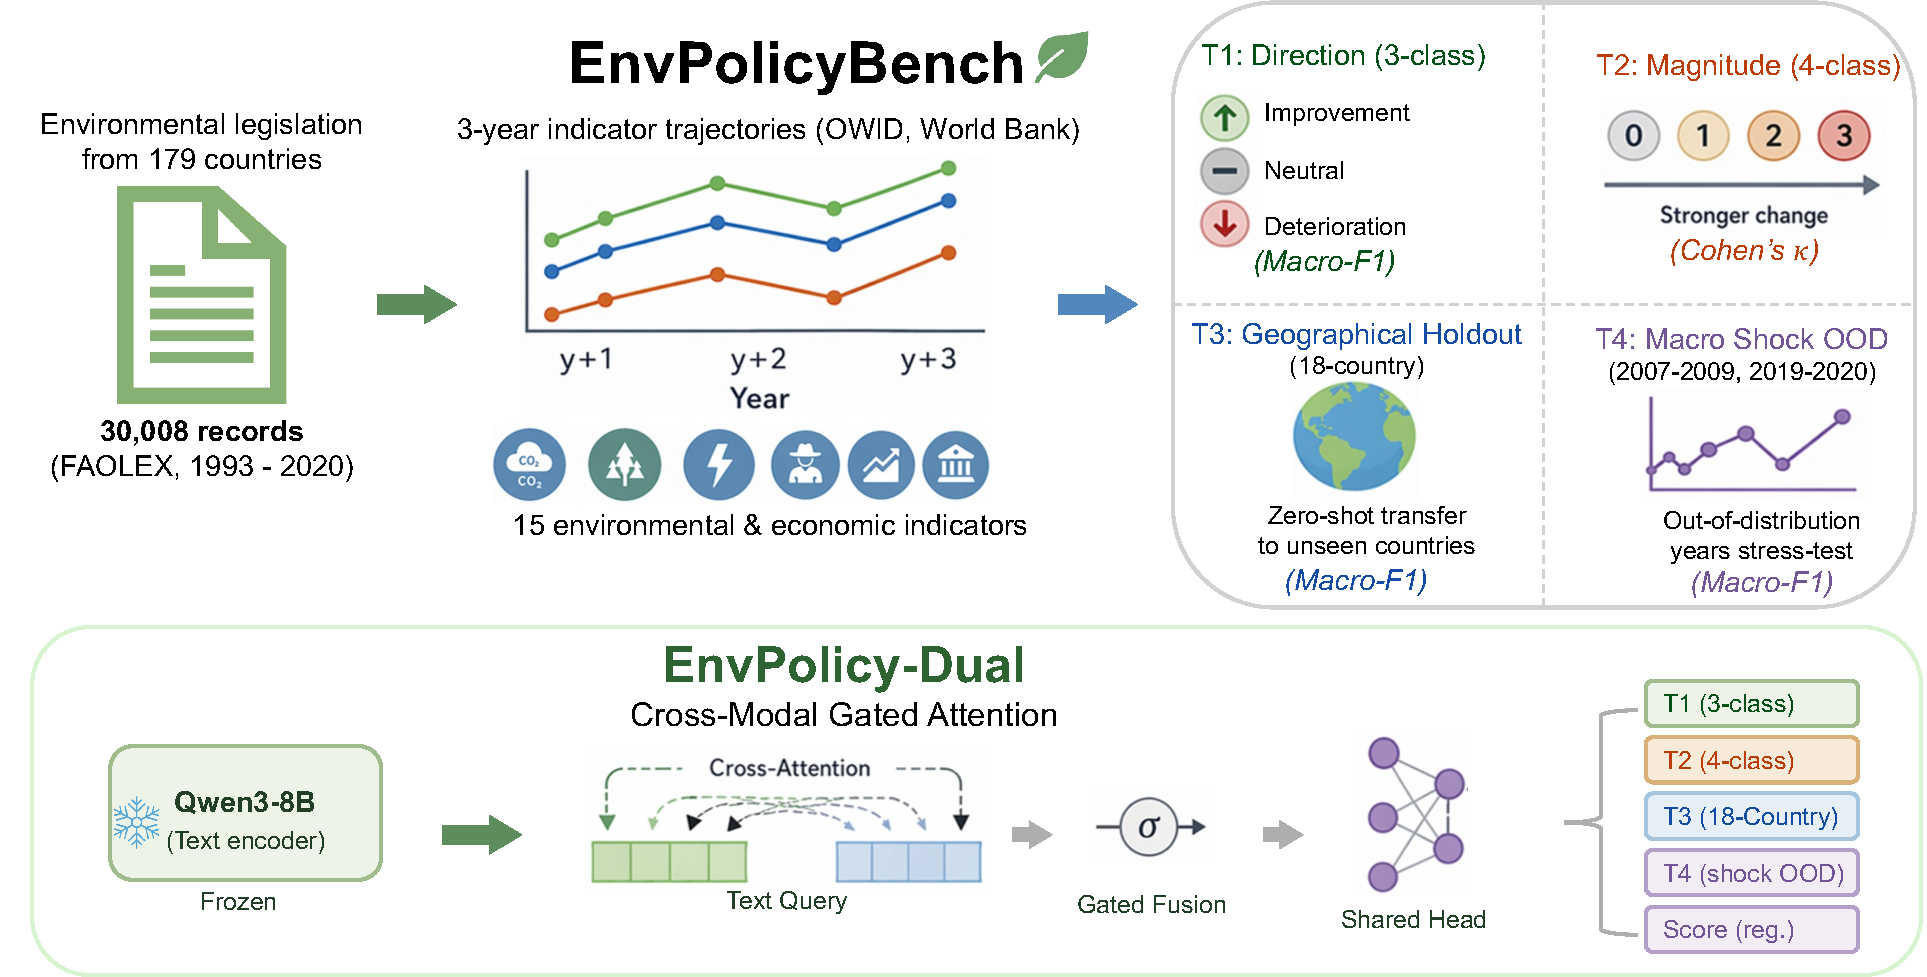
\includegraphics[width=0.9\linewidth]{figures/Fig_method.pdf}
    \caption{EnvPolicyBench dataset and EnvPolicy-Dual model architecture for multi-task environmental policy impact prediction across direction, magnitude, geographical, and out-of-distribution macro-shock settings.}
    \label{fig:placeholder}
\end{figure*}


\subsection{Multimodal and Structured Feature Fusion}

The core of our approach is to combine  unstructured text with structured tabular features. Prior studies in finance and healthcare have explored fusion of text and structured data using neural architectures, including FinBERT-style models \citep{yang2020finbert}, multi-task fusion networks \citep{sawhney2021finmtl}, and multimodal learning \citep{khadanga2019sensefusion}. When the modalities are noisy or missing, cross-modal attention mechanisms \citep{tsai2019multimodal} and gated fusion strategies \citep{arevalo2017gated} have been shown to improve robustness.

We adapt the above ideas to this research, in which long-text documents should be aligned with environmental indicator series. \bench{} is distinct in combining labels derived from real post-enactment indicator trajectories rather than human annotation. The dataset covers 179 countries and 30{,}000 records with a leakage-free split. Furthermore, geographic (T3, 18-country holdout) and temporal (T4, macro-shock) out-of-distribution evaluations are introduced. 


\section{The \bench{} Dataset}
\label{sec:dataset}

\subsection{Data Sources}
\label{sec:data-sources}

\paragraph{Legislative records.}
We collect policy records from the FAO \textsc{Faolex} database \citep{faolex2024}.  In this study,  only English-language entries are retained with titles and abstracts passing a language identification filter and whoseyear\_enacted falls between 1993 and 2020. After that, the data is cleaned to remove the recodes if country ISO codes mismatch, or if fewer than two years of post-enactment indicator data are available. As a result, each document is constructed by connecting the title, long title, and summary, which is further truncated to 512 WordPiece tokens for standardized processing.

\paragraph{Environmental and economic indicators.}
We combine the OWID dataset \citep{owid-co2},  World Bank (WB) World Development Indicators (WDI) \citep{worldbank} and FAOSTAT \citep{faostat}. The resulting panel includes GDP per capita, renewable energy share, forest area share, agricultural value added share, rural population share, food insecurity rate, trade openness, industry value added share, and government final consumption share. All time series are harmonized to ISO-3 country identifiers and aligned at the yearly level.

\paragraph{Feature set.}
Table~\ref{tab:features} summarizes the 15-dimensional pre-enactment feature vector constructed for each (country, year) pair. The features capture indicators before policy. Missing values are handled using a validity mask $m \in \{0,1\}^{15}$, paired with zero imputation, following practice in tabular deep learning \citep{van2023missing}.


\begin{table}[!t]
\centering\small
\setlength{\tabcolsep}{3pt}
\resizebox{\columnwidth}{!}{
\begin{tabular}{@{}p{2cm}p{6.4cm}@{}}
\toprule
\textbf{Category} & \textbf{Features} \\
\midrule

Environmental (12 features) &
CO$_2$ per capita; CO$_2$ growth rate; GHG per capita; fossil fuel share; renewable energy share; energy use per capita; food insecurity rate; agricultural emissions; GDP per capita; agricultural value added share; forest area share; rural population share \\

\midrule

Macroeconomic (3 features) &
Trade openness; industry value added share; government final consumption share \\

\bottomrule
\end{tabular}}
\caption{Pre-enactment feature set used for each (country, year) observation.}
\label{tab:features}
\end{table}



\subsection{Alignment Pipeline}
\label{sec:pipeline}


The alignment procedures are shown in Algorithm~\ref{alg:align}. For each policy in year $y$ and country $c$, we construct a pre-enactment indicator vector using data from year $y-1$. Then a post-enactment outcome window covering years $\{y+1, y+2, y+3\}$ is defined to capture changes following policy adoption. Records with fewer than two years of valid post-enactment indicator data are excluded. The above procedures ensure sufficient coverage for reliable outcome estimation and reduce bias.

\begin{algorithm}[t]
\small
\caption{Policy–Outcome Alignment}
\label{alg:align}
\begin{algorithmic}[1]
\Require Legal records $\mathcal{R}$, indicator tables $\mathcal{I}$
\Ensure Aligned dataset $\mathcal{D}$
\State $\mathcal{D}\gets\emptyset$
\ForAll{$r\in\mathcal{R}$}
    \State $(c,y)\gets(r.\text{iso3}, r.\text{year})$
    \State $x\gets \mathcal{I}[c, y-1]$ \Comment{15 features + mask $m$}
    \If{$x$ is undefined or $\|m\|_1 < \tau d$}
    \State \textbf{continue}
    \EndIf
    \State $\{\tilde{x}_k\}_{k=1}^{3}\gets \mathcal{I}[c, y+k]$
    \State $s_r \gets \textsc{CompositeScore}(x, \{\tilde{x}_k\})$
    \State $(y^{T1}_r, y^{T2}_r)\gets\textsc{Labels}(s_r)$
    \State $\mathcal{D}\gets\mathcal{D}\cup\{(r.\text{text}, x, m, y^{T1}_r, y^{T2}_r, s_r)\}$
\EndFor
\State \textbf{return} $\mathcal{D}$
\end{algorithmic}
\end{algorithm}

\subsection{Label Design}
\label{sec:labels}

\paragraph{Composite score.}
Following standard composite indicator construction and environmental accounting practices \citep{joint2008handbook}, we construct an environmental outcome score to measure the effect of the legislative enactment. To avoid cross-sector aggregation bias, we restrict evaluation to domain-relevant indicators. Table~\ref{tab:domain_inds} shows domain-specific positive and negative indicator sets $P_D$ and $N_D$, based on common environmental economics conventions.  These mappings are validated with domain experts to ensure alignment between policy intent and measurable environmental outcomes.

Given a record $r$ with inferred domain $D$, the composite score is defined as:
\begin{equation}
s_r = \frac{1}{|P_D|}\sum_{p \in P_D} \tilde{\Delta}^{3y}_{p}
    - \frac{1}{|N_D|}\sum_{n \in N_D} \tilde{\Delta}^{3y}_{n},
\label{eq:composite}
\end{equation}
where $\tilde{\Delta}^{3y}$ is the normalized three-year post-enactment change. Higher positive and lower negative indicators indicate better effectiveness.

\begin{table}[!t]
\centering\small
\setlength{\tabcolsep}{3pt}
\resizebox{\columnwidth}{!}{%
\begin{tabular}{@{}lp{3.5cm}p{4.5cm}@{}}
\toprule
\textbf{Domain} & \textbf{Positive ($P_D$)} & \textbf{Negative ($N_D$)} \\
\midrule
Energy      & renewables share & fossil share, CO$_2$/cap, GHG/cap, CO$_2$ growth \\
Environment & renewables, forest & CO$_2$/cap, GHG/cap, fossil, CO$_2$ growth \\
Agriculture & agri.\ value added, forest & agri.\ GHG (kt) \\
Fisheries   & GDP/cap & food insecurity \% \\
Food Safety & GDP/cap & food insecurity \% \\
Land/Water  & forest, agri.\ value added & CO$_2$/cap \\
Other       & renewables, forest & CO$_2$/cap, GHG/cap \\
\bottomrule
\end{tabular}%
}
\caption{Domain-specific indicator groups used for composite outcome scoring.}
\label{tab:domain_inds}
\end{table}

\textit{Pseudo-DiD regional baseline.}
To reduce contamination from macro-economic shocks that affect all countries
simultaneously, we subtract the regional median
3-year delta from each indicator before computing the composite score:
\begin{equation}
\widetilde{\Delta}^{3y}_{k,r}
  = \Delta^{3y}_{k,r} - \operatorname{median}_{r'\in\text{region}(r)}\!\!\Delta^{3y}_{k,r'},
\label{eq:pseudo_did}
\end{equation}
producing a \emph{relative} indicator change $\widetilde{\Delta}$ that
approximates a difference-in-differences estimator with regional peers as
the counterfactual.

\textit{Normalisation.}
To prevent any single high-variance indicator from dominating, we apply
per-indicator winsorisation at the [1\%, 99\%] quantiles computed on unique
country-year pairs, then z-score normalise each winsorised variable using its
country-year-level mean and standard deviation ($\tilde{\Delta}^{3y}_{k}$ in
Eq.~\ref{eq:composite}).
\textcolor{red}{The normalisation parameters (winsorise bounds, mean, std per indicator) are
saved to \texttt{norm\_params.json} for reproducible inference.}

\paragraph{T1 (direction).}
We apply data-driven thresholds $\theta^{+}=+0.05$ and $\theta^{-}=-0.05$ to
$\{s_r\}$: scores above $\theta^{+}$ receive label \textsf{improvement},
scores below $\theta^{-}$ receive \textsf{deterioration}, and the remainder
receive \textsf{neutral}. The resulting distribution is 56.4\% improvement,
10.2\% neutral, 33.4\% deterioration. Such processing produces a more balanced prior than the
un-normalised version. And this also reflects the real-world macroeconomic dynamics.

\paragraph{T2 (magnitude).}
Absolute score thresholds map to four classes: $|s|<0.05$ (class 0, neutral),
$0.05 \le |s|<0.2199$ (class 1, mild), $0.2199 \le |s|<0.4874$ (class 2,
moderate), $|s|\ge0.4874$ (class 3, strong). Thresholds are calibrated
so that classes 1--3 each contain approximately equal numbers of non-neutral
records (T2 distribution: 10.2 / 29.6 / 30.5 / 29.7\%).

\paragraph{Label quality metadata.}
Two auxiliary fields accompany each record to enable quality-stratified evaluation.
\textbf{label\_confidence} reflects the fraction of domain-relevant ($P_D \cup N_D$)
indicators that carry valid (non-NaN) values for the record's country-year:
\textit{high} ($\ge$66\%), \textit{medium} ($\ge$33\%), or \textit{low} ($<$33\%).
Researchers may restrict evaluation to the high-confidence subset for a less noisy
but smaller benchmark.
\textbf{label\_consistent} is a Boolean flag that is True when
the T1 direction label derived from the 3-year composite score agrees with the
label derived from the analogous 5-year window. Records with label\_consistent=True
form a ``gold'' sub-benchmark where the label signal is stable across time horizons.
\textcolor{red}{Both fields are present in all released split files and can be used as filters at
evaluation time without altering the benchmark splits themselves.}

\paragraph{T3 (cross-country transfer).}
We additionally produce a country-holdout split by selecting 18 countries---3
per geographic region, stratified to include a range of record counts---and
moving all their records to a held-out test set (2{,}523 records). Training on
the remaining 159 countries and testing on the held-out 18 measures zero-shot
geographic transfer and penalizes models that learn country priors instead of
reading the law text.

\subsection{Statistics}
\label{sec:stats}

\paragraph{Quality filter and dataset provenance.}
As shown in Table~\ref{tab:stats}, we begin with 31{,}404 English-language FAOLEX records and apply a \textit{domain-aligned quality filter}: a record is retained only if the composite score $s_r$ is computable. This removes 4.4\% of records (1{,}396), yielding \textbf{30{,}008 records}. For retained records, 97.9\% have label\_confidence=high and 2.1\% =medium; no low-confidence records survive. Additionally, 69.2\% of eligible records have label\_consistent=True, forming a gold sub-benchmark of 19{,}446 records. The remaining 1{,}894 records (policy year $\ge$2019) carry label\_consistent=NaN because the 5-year window exceeds the data time range. Furthermore, we formalize the results as follows: \textbf{Gold} (label\_consistent=True, 64.8\%), \textbf{Silver} (high/medium confidence but consistent disagrees, 35.2\%), and \textbf{Bronze} (low confidence; 0 records in this release, as no low-confidence records survive the filter). Additionally, 21.2\% of records carry is\_amendment=1,
derived solely from a case-insensitive title-pattern match (\textbackslash bamend); we do \emph{not} use the FAOLEX last\_amended field for this purpose because that field identifies \emph{original} laws that were subsequently amended by another document, not the amending document itself.  

The domain distribution spans agriculture (25.3\%), environment-proper (22.2\%), food safety (18.8\%), fisheries (15.3\%), land/water (9.9\%), energy (4.8\%), and other (3.8\%). Regional coverage is Europe (34.2\%), Asia (23.6\%), Africa (15.3\%), Oceania (13.6\%), Americas (10.9\%).

\begin{table}[t]
\centering\small
\resizebox{\columnwidth}{!}{%
\begin{tabular}{@{}lr@{}}
\toprule
\textbf{Property} & \textbf{Value} \\
\midrule
Raw FAOLEX records (English)  & 31{,}404 \\
After domain-aligned quality filter & 30{,}008 \\
Countries / ISO-3 codes       & 179 \\
Year range                    & 1993--2020 \\
Mean text length (tokens)     & 186 \\
Indicator dim.\ / mask dim.   & 15 / 15 \\
Domain-relevant indicators (per domain) & 2--5 \\
\midrule
Train / Val / Test            & 17{,}704 / 2{,}166 / 1{,}826 \\
Split level                   & country-year group \\
Random-split seed             & 42 \\
Country-holdout test (T3)     & 18 countries, 2{,}523 records \\
\midrule
\texttt{label\_tier}: Gold / Silver / Bronze & 64.8 / 35.2 / -- \\
Multilingual records (fr+es)  & $\sim$60{,}000 (separate file) \\
Amendment records (\texttt{is\_amendment=1}) & $\sim$21\% \\
\midrule
T1: imp / neu / det (\%)      & 56.4 / 10.2 / 33.4 \\
T1 train / val / test (\% imp)$^\dagger$ & 60.6 / 52.2 / 46.8 \\
T2: class 0/1/2/3 (\%)        & 10.2 / 29.6 / 30.5 / 29.7 \\
\bottomrule
\end{tabular}%
}
\caption{\bench{} dataset statistics.}
\label{tab:stats}
\end{table}

\subsection{Task Definition}
\label{sec:tasks}

Given a record $r=(\text{text}_r, x_r, m_r)$, where $x_r$ contains pre-enactment indicators and $m_r$ is the corresponding validity mask, models need to predict the direction and magnitude observed in the country during the three years after policy enactment.

Formally: \textbf{T1} $y^{T1}_r\in\{imp,neu,det\}$, scored by macro-F1 and macro-AUC; \textbf{T2} $y^{T2}_r\in\{0,1,2,3\}$, scored by macro-F1 and quadratic weighted Cohen's $\kappa$ (to reward ordinal closeness); and \textbf{T3}, the same labels evaluated on the 18-country holdout set, with performance drop $\Delta$ relative to the main test split as the primary metric.

%\textcolor{red}{Auxiliary regression on the composite score $s_r$ is reported with Spearman $\rho$ and mean absolute error (MAE).} 

The use of post-$y$ indicator values is forbidden to exclude label leakage. All three tasks are framed as associational outcome prediction. The labels reflect country-level macro-environmental trajectories, but not the causal effect of individual policies. T3 forces models to rely on the legal text rather than memorized country priors.


\section{The \ours{} Model}
\label{sec:model}

\subsection{Architecture}

\ours{} has three sub-networks motivated by the complementary nature of the two modalities: a text encoder, an indicator encoder, and a cross-modal fusion module.

\paragraph{Text encoder.}
Qwen3-8B \citep{qwen2025} with frozen weights is as the text encoder. The pooled last-hidden-state serves as the text representation:
\begin{equation}
\mathbf{h}_t = \text{Qwen3-8B}(\text{text}_r)_{\text{pool}}\in\mathbb{R}^{4096}.
\end{equation}
Only the fusion layers and task heads are trained (2.09M trainable parameters), while the text encoder is kept frozen to avoid catastrophic forgetting on the relatively small training set.

\paragraph{Indicator encoder.}
Normalized indicators $x$ and validity mask $m$ are combined by an elementwise product and fed to a two-layer MLP:
\begin{equation}
\mathbf{h}_i = \text{LN}\!\bigl(\text{GELU}(W_2\,\text{GELU}(W_1(x\odot m)))\bigr)\in\mathbb{R}^{128}.
\end{equation}
$W_1\in\mathbb{R}^{64\times 15}$, $W_2\in\mathbb{R}^{128\times 64}$, each followed by dropout $p=0.1$. Multiplying by $m$ before the first linear layer, ensuring that missing indicators propagate as zero activations rather than fake signals.

\paragraph{Cross-modal fusion.}
Both streams are projected to a common dimension $d=256$: $\mathbf{t}'\!=\!W_t\mathbf{h}_t$, $\mathbf{i}'\!=\!W_i\mathbf{h}_i$. A single-head cross-attention
lets the text \emph{query} the indicator stream:
\begin{align}
\mathbf{a}\;&=\;\text{softmax}\!\Big(\tfrac{\mathbf{t}'W_Q(\mathbf{i}'W_K)^{\!\top}}{\sqrt{d}}\Big)\mathbf{i}'W_V,\\
\mathbf{g}\;&=\;\sigma(W_g[\mathbf{t}';\mathbf{a}]),\\
\mathbf{f}\;&=\;\mathbf{g}\odot\mathbf{a}+(1-\mathbf{g})\odot\mathbf{t}',\\
\mathbf{z}\;&=\;\text{FFN}(\text{LN}(\mathbf{f})).
\end{align}
The gate $\mathbf{g}$ learns when to trust indicators over text. This can mitigate noise from countries with sparse numeric coverage. We argue this \emph{text-queries-indicator} direction is natural: the law specifies the policy domain, which determines which economic signals are most relevant.

\paragraph{Task heads.}
A 3-way, 4-way, and scalar head share $\mathbf{z}$:
$\ell^{T1}\!=\!\text{H}_{1}(\mathbf{z})$,
$\ell^{T2}\!=\!\text{H}_{2}(\mathbf{z})$,
$\hat{s}\!=\!\text{H}_{\text{reg}}(\mathbf{z})$.

\subsection{Training Objective}

\begin{equation}
\mathcal{L} = \mathcal{L}_{\text{CE}}^{T1} + \mathcal{L}_{\text{CE}}^{T2}
            + \lambda_r\,\mathcal{L}_{\text{SmoothL1}}(\hat{s},\,s)
            + \lambda_c\,\mathcal{L}_{\text{NT-Xent}},
\label{eq:loss}
\end{equation}
with $\lambda_r\!=\!0.5$, $\lambda_c\!=\!0.1$, NT-Xent temperature
$\tau\!=\!0.07$, and positive pairs are defined as records sharing (country, domain, T1-label) in the same minibatch \citep{chen2020simclr}. Class weights inversely proportional to frequency are applied to both CE losses to address the skewed T1 and T2 distributions. The contrastive term structures the fused
representation so that policies with similar context and outcome cluster together, which we found especially beneficial for T3.

\subsection{Training Details}

We use AdamW with a OneCycleLR scheduler. The batch size is 16, and the learning rate is  $2\!\times\!10^{-5}$ for the pretrained text encoder and $1\!\times\!10^{-4}$ for MLP and heads. Warmup is 10\%, and weight decay is 0.01. The indicator-only MLP is trained to full convergence on the complete training set. \ours{} uses the
full training set (17{,}704 records) with the Qwen3-8B encoder frozen (only fusion layers and task heads are trained (2.09M parameters)). All hyperparameters are selected on the validation set.

\section{Experiments}
\label{sec:exp}

\subsection{Baselines}

We evaluate 27 zero-shot LLMs spanning 8 model families (Table~\ref{tab:models}),
plus feature-based and fine-tuned baselines.

\begin{table}[!t]
\centering\small
\setlength{\tabcolsep}{4pt}
\begin{tabular}{@{}ll@{}}
\toprule
\textbf{Family} & \textbf{Models} \\
\midrule
OpenAI      & GPT-5, GPT-5-mini, GPT-5.1, GPT-5.2, GPT-5.5 \\
Anthropic   & Claude Sonnet 4.5, Opus 4.5, Opus 4.7 \\
Google      & Gemini 2.5 Pro/Flash, 3 Pro/Flash, 3.1 Pro \\
DeepSeek    & DeepSeek-R1, V3, V3.2, V4-Pro \\
ByteDance   & Doubao Seed 1.6, 2.0-Lite, 2.0-Pro \\
Moonshot    & Kimi-K2.5 \\
Others      & GLM-5, GLM-5.1, MiniMax-M2.5, Qwen3.6-Plus, \\
            & Hunyuan-3 \\
\bottomrule
\end{tabular}
\caption{Zero-shot LLM families evaluated (27 models total).}
\label{tab:models}
\end{table}

\noindent Feature-based and fine-tuned baselines:
\textbf{TF-IDF + LR}: bag-of-words TF-IDF (1--2 gram, 50k features, sublinear TF, min\_df=3) with Logistic Regression (C=1.0, lbfgs solver, trained on full 17{,}704 records).
\textbf{TF-IDF + RF}: same TF-IDF features with a Random Forest (200 trees, max\_depth=20).
\textbf{Indicator-only MLP}: the indicator branch of \ours{} with a single classification head, trained to convergence on all 17{,}704 records.
\textbf{Qwen3-8B (text-only)}: Qwen3-8B encoder with a classification head, no indicator input; trained on full training set with frozen encoder.
\textbf{Qwen3-8B (SFT)}: Qwen3-8B supervised fine-tuned end-to-end on text classification (T1 only).

\subsection{Main Results}

%% table_llm_zeroshot.tex
%% Zero-shot LLM baselines
\begin{table*}[!t]
\centering\footnotesize
\setlength{\tabcolsep}{4pt}
\setlength{\fboxsep}{1.5pt} % reduced padding to fix number position
\definecolor{bestcell}{RGB}{255,235,156}
\definecolor{secondcell}{RGB}{189,215,238}
\begin{tabular}{@{}l rrr rr r rr@{}}
\toprule
 & \multicolumn{3}{c}{\textbf{T1 Direction (Test)}}
 & \multicolumn{2}{c}{\textbf{T2 Magnitude (Test)}}
 & \textbf{T3 Holdout}
 & \multicolumn{2}{c}{\textbf{T4 OOD (Shock yrs)}} \\
\cmidrule(lr){2-4}\cmidrule(lr){5-6}\cmidrule(lr){7-7}\cmidrule(lr){8-9}
\textbf{Model}
  & \textbf{Acc}$\uparrow$
  & \textbf{F1}$\uparrow$
  & $\boldsymbol{\kappa}\uparrow$
  & \textbf{F1}$\uparrow$
  & \textbf{MAE}$\downarrow$
  & \textbf{F1}$\uparrow$
  & \textbf{Acc}$\uparrow$
  & \textbf{F1}$\uparrow$ \\
\midrule
\multicolumn{9}{l}{\textit{OpenAI}} \\
GPT-5 & \colorbox{bestcell}{\textbf{0.343}} & 0.276 & \colorbox{bestcell}{\textbf{0.015}} & 0.154 & 1.331 & 0.264 & \colorbox{secondcell}{0.367} & 0.284 \\
GPT-5-mini & 0.317 & 0.275 & $-$0.024 & 0.173 & 1.203 & 0.251 & 0.333 & 0.279 \\
GPT-5.1 & 0.311 & 0.261 & $-$0.033 & 0.182 & 1.092 & 0.269 & 0.347 & 0.307 \\
GPT-5.2 & 0.305 & 0.249 & $-$0.042 & 0.194 & 1.106 & 0.270 & 0.339 & 0.278 \\
GPT-5.5 & 0.301 & 0.243 & $-$0.048 & 0.226 & 1.115 & 0.247 & 0.353 & 0.285 \\
\midrule
\multicolumn{9}{l}{\textit{Anthropic}} \\
Claude Sonnet 4.5 & 0.317 & 0.278 & $-$0.024 & 0.188 &  \colorbox{bestcell}{\textbf{1.068}} & 0.278 & 0.353 & 0.310 \\
Claude Opus 4.5 & 0.293 & 0.230 & $-$0.060 & 0.209 & 1.141 & 0.231 & 0.326 & 0.257 \\
Claude Opus 4.6 & 0.293 & 0.227 & $-$0.060 & 0.203 & 1.129 & 0.227 & 0.326 & 0.253 \\
Claude Opus 4.7 & 0.319 & 0.263 & $-$0.021 & 0.201 & 1.100 & 0.263 & 0.355 & 0.293 \\
\midrule
\multicolumn{9}{l}{\textit{Google Gemini}} \\
Gemini 2.5 Flash & 0.315 & 0.268 & $-$0.027 &  \colorbox{bestcell}{\textbf{0.243}}  & 1.213 & 0.270 & 0.355 & 0.291 \\
Gemini 2.5 Pro & 0.321 & 0.283 & $-$0.018 & \colorbox{secondcell}{0.242} & 1.229 & \colorbox{bestcell}{\textbf{0.295}} & 0.355 & 0.308 \\
Gemini 3 Pro & 0.313 & 0.259 & $-$0.030 & 0.215 & 1.203 & 0.255 & 0.355 & 0.298 \\
Gemini 3 Flash & 0.311 & 0.226 & $-$0.033 & 0.205 & 1.149 & 0.202 & 0.353 & 0.272 \\
Gemini 3.1 Pro & 0.297 & 0.243 & $-$0.054 & 0.225 & 1.195 & 0.254 & 0.353 & 0.296 \\
\midrule
\multicolumn{9}{l}{\textit{DeepSeek}} \\
DeepSeek-R1 & 0.311 & \colorbox{secondcell}{0.283} & $-$0.033 & 0.207 & 1.145 & 0.290 & 0.343 & 0.302 \\
DeepSeek-V3 & 0.299 & 0.241 & $-$0.051 & 0.185 &  \colorbox{secondcell}{1.076}  & 0.248 & 0.351 & 0.289 \\
DeepSeek-V3.2 & 0.303 & 0.259 & $-$0.045 & 0.221 & 1.167 & 0.262 & \colorbox{bestcell}{\textbf{0.369}} & \colorbox{bestcell}{\textbf{0.317}} \\
DeepSeek-V4-Pro & 0.321 & 0.277 & $-$0.018 & 0.222 & 1.167 & 0.278 & 0.353 & \colorbox{secondcell}{0.316} \\
\midrule
\multicolumn{9}{l}{\textit{ByteDance (Doubao)}} \\
Doubao Seed 1.6 & 0.327 & 0.269 & $-$0.009 & 0.218 & 1.145 & 0.234 & 0.335 & 0.274 \\
Doubao Seed 2.0 Lite & 0.311 & 0.260 & $-$0.033 & 0.196 & 1.153 & 0.233 & 0.333 & 0.265 \\
Doubao Seed 2.0 Pro &  \colorbox{secondcell}{0.329} & 0.257 & \colorbox{secondcell}{$-$0.006} & 0.203 & 1.169 & 0.231 & 0.357 & 0.278 \\
\midrule
\multicolumn{9}{l}{\textit{Other}} \\
Kimi-K2.5 & 0.321 & \colorbox{bestcell}{\textbf{0.293}} & $-$0.018 & 0.146 & 1.201 & 0.288 & 0.317 & 0.285 \\
GLM-5 & 0.321 & 0.208 & $-$0.018 & 0.140 & 1.121 & 0.208 & 0.345 & 0.245 \\
GLM-5.1 & 0.305 & 0.219 & $-$0.042 & 0.171 & 1.217 & 0.245 & 0.337 & 0.244 \\
MiniMax M2.5 & 0.311 & 0.268 & $-$0.033 & 0.194 & 1.267 & \colorbox{secondcell}{0.294} & 0.335 & 0.277 \\
Qwen3.6-Plus & 0.297 & 0.247 & $-$0.054 & 0.201 & 1.203 & 0.257 & 0.341 & 0.284 \\
Hunyuan 3 & 0.303 & 0.255 & $-$0.045 & 0.207 & 1.468 & 0.282 & 0.359 & 0.302 \\
\midrule
\multicolumn{9}{l}{\textit{Supervised reference}} \\
TF-IDF + LR & 0.533 & 0.364 & $\phantom{-}$0.145 & 0.242 & 1.632 & 0.341 & 0.498 & 0.338 \\
Indicator-only MLP & 0.466 & 0.419 & $\phantom{-}$0.191 & 0.129 & 0.306 & 0.371 & 0.441 & 0.389 \\
\textbf{EnvPolicy-Dual} & \textbf{0.596} & \textbf{0.412} & $\phantom{-}$\textbf{0.281} & \textbf{0.225} & \textbf{0.987} & \textbf{0.382} & \textbf{0.562} & \textbf{0.386} \\
\bottomrule
\end{tabular}
\caption{Zero-shot LLM evaluation on T1 direction, T2 magnitude, T3 geographic holdout (18-country zero-shot),
and T4 temporal OOD (shock years 2007--2009, 2019--2020). Stratified sample $ n $=498 per split.
Models grouped by family, ordered by version.
\colorbox{bestcell}{\textbf{Yellow}} = best; \colorbox{secondcell}{blue} = second best among LLMs.}
\label{tab:llm_zeroshot}
\end{table*}

\begin{table*}[!t]
\centering
\small
\resizebox{\textwidth}{!}{%
\begin{tabular}{lcccccccc}
\toprule
\textbf{Model}
  & \textbf{T1 F1}$\uparrow$
  & \textbf{T1 $\kappa$}$\uparrow$
  & \textbf{T1 Acc}$\uparrow$
  & \textbf{T2 F1}$\uparrow$
  & \textbf{T2 $\kappa$}$\uparrow$
  & \textbf{T2 MAE}$\downarrow$
  & \textbf{T3 F1}$\uparrow$
  & \textbf{T4 F1}$\uparrow$ \\
\midrule
\multicolumn{9}{l}{\textit{Zero-shot Baselines}} \\
Qwen3-8B (zero-shot)        & 0.206 & $-$0.042 & 0.301 & 0.148 & $-$0.031 & 1.285 & 0.194 & 0.218 \\
Best LLM (Kimi-K2.5)        & 0.293 & $-$0.018 & 0.321 & 0.146 & $-$0.053 & 1.201 & 0.288 & 0.285 \\
\midrule
\multicolumn{9}{l}{\textit{Feature-based Baselines }} \\
TF-IDF + LR                 & 0.364 & 0.145    & 0.533 & \textbf{0.242} & 0.015 & 1.632 & 0.341 & 0.338 \\
TF-IDF + RF                 & 0.298 & 0.076    & 0.475 & 0.226 & 0.009 & 1.456 & 0.275 & 0.281 \\
Indicator-only MLP          & \textbf{0.419} & 0.191 & 0.466 & 0.129 & $-$0.100 & \textbf{0.306} & 0.371 & 0.389 \\
\midrule
\multicolumn{9}{l}{\textit{Supervised Fine-tuned }} \\
Qwen3-8B (SFT, T1 only)$^\dag$    & 0.388 & 0.000    & 0.502 & \multicolumn{3}{c}{(T1 only)} & 0.362 & 0.355 \\
Qwen3-8B (text-only, dual)$^\dag$  & 0.213 & 0.000    & 0.468 & 0.127 & $-$0.068 & 1.342 & 0.198 & 0.225 \\
\midrule
\multicolumn{9}{l}{\textit{Our Model }} \\
\textbf{EnvPolicy-Dual (Qwen3-8B)}$^\dag$
                            & 0.412 & \textbf{0.281} & \textbf{0.596} & 0.225 & \textbf{0.048} & 0.987 & \textbf{0.382} & \textbf{0.386} \\
\bottomrule
\end{tabular}%
}
\caption{Main results on EnvPolicyBench test set ($n$=1{,}826).
T1 = direction (3-class); T2 = magnitude (4-class);
T3 = 18-country geographic holdout ($n$=2{,}523); T4 = temporal OOD, shock years ($n$=5{,}789).
Bold = best per column.
$^\dag$Qwen3-8B frozen encoder, 2.09\,M trainable parameters.
Full 27-model LLM comparison in Table~\ref{tab:llm_zeroshot}.}
\label{tab:main_results}
\end{table*}


Table~\ref{tab:llm_zeroshot} reports zero-shot LLM results across all 27 models
on T1, T2, and the T4 OOD split. Table~\ref{tab:main_results} compares
feature-based, fine-tuned, and our cross-modal model.
We highlight four findings.

\textbf{Lexical signal is surprisingly strong.} TF-IDF + LR achieves T1 macro-F1 of 0.364 and T1 AUC of 0.607. It suggests that titles and abstracts carry a discriminative signal about eventual outcomes. Notably, the indicator-only MLP surpasses TF-IDF + LR on T1 (0.419 vs.\ 0.364), despite working only from a numeric economic context.

\textbf{Indicators and text encode complementary information.} The indicator-only MLP achieves better MAE (0.306 vs.\ 1.632 for TF-IDF+LR) on the continuous regression target, because the raw score $s_r$ is numerically related to the indicator deltas it is trained against. However, the MLP fails on T2 classification ($\kappa=-0.100$) and only narrowly beats TF-IDF + LR on T1 F1 (0.419 vs.\ 0.364), indicating that without reading the policy text, indicator context cannot reliably determine whether a policy will
shift outcomes in a positive direction. This is the core motivation for \ours.


\textbf{Zero-shot LLMs fall below lexical baselines.}
Twenty-seven frontier LLMs (spanning GPT-5/5.1/5.2/5.5, Claude Sonnet/Opus 4.x, Gemini 2.5/3.x, DeepSeek-R1/V3/V4-Pro, Kimi-K2.5, and others) are evaluated zero-shot on T1 and T2 (Table~\ref{tab:llm_zeroshot}). The best macro-F1=0.293 (Kimi-K2.5) , well below TF-IDF+LR (0.364). Most $\kappa$ values are negative across all LLM models, indicating performance close to random guessing.

\textbf{Universal optimism bias.}
Every model exhibits a systematic \emph{improvement bias}: recall for the
\textit{improvement} class exceeds 0.53, while recall for \textit{deterioration}
falls below 0.13. Reasoning-augmented models (GPT-5.1, DeepSeek-R1, Gemini 2.5)
do not outperform standard chat models, confirming that chain-of-thought cannot
recover missing post-enactment outcome knowledge.

\subsection{Cross-Country Transfer (T3) and Temporal OOD (T4)}

On the 18-country holdout ($n{=}2{,}523$), most LLMs show modest degradation: Kimi-K2.5 shows the smallest drop (F1 $0.293\!\to\!0.288$, $\Delta{=}{-}0.005$) while Doubao Seed 1.6 degrades most ($0.269\!\to\!0.234$, $\Delta{=}{-}0.036$). A small number of models (e.g.\ Gemini 2.5 Flash, $\Delta{=}{+}0.002$) show marginal improvement, suggesting robustness to geographic distribution shift varies by model family.

An interesting finding from T4 OOD (Table~\ref{tab:llm_zeroshot}) is that several models perform \emph{better} on the shock-year split than on the in-distribution test (e.g.\ DeepSeek-V3.2: test F1=0.259 vs.\ T4 F1=0.317). This suggests LLMs may have stronger priors about policy effects during extreme events (financial crises, pandemics),  where outcomes are more salient in their training corpora.

\begin{figure}[t]
    \centering
    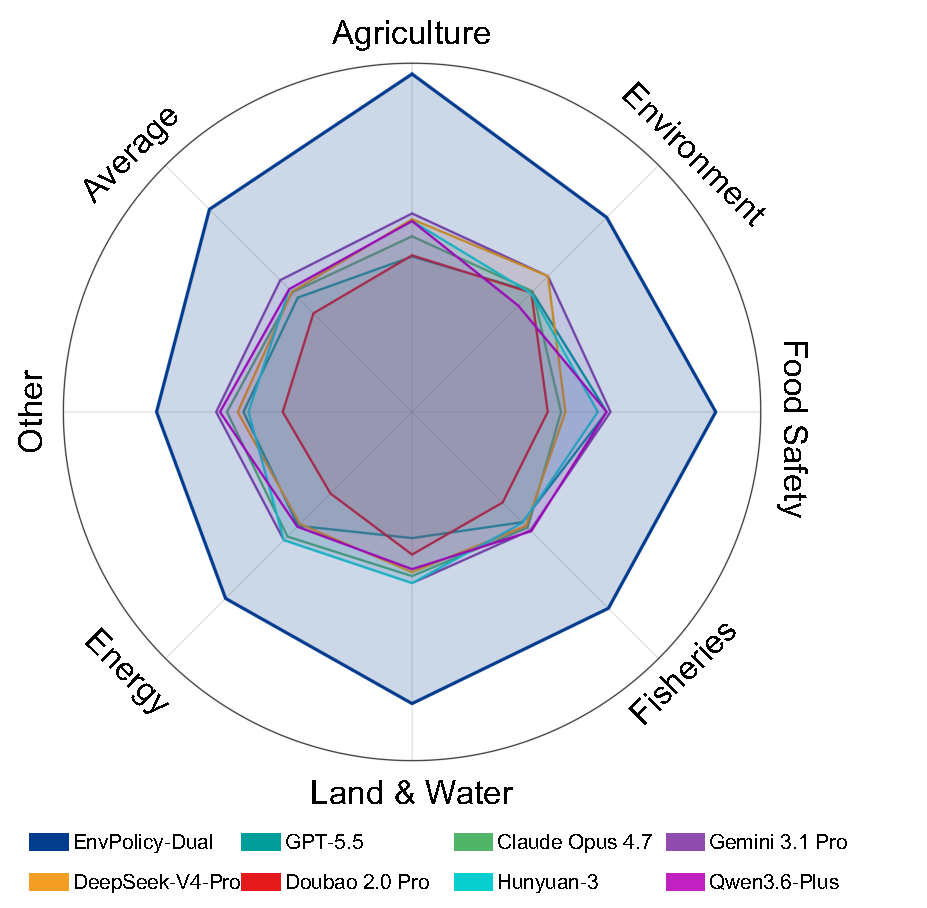
\includegraphics[width=0.9\linewidth]{figures/Domain performance.pdf}
    \caption{Domain-level comparison of T1 Macro-F1 performance across environmental policy categories. Detailed values can be found in Appendix~\ref{app:domain_breakdown}. }
    \label{fig:domain_break}
\end{figure}


\subsection{Ablation}

\begin{table}[t]
\centering\small
\begin{tabular}{@{}lcc@{}}
\toprule
\textbf{Variant} & \textbf{T1 F1} & \textbf{T2 F1} \\
\midrule
\ours{} full                           & \textbf{0.412} & \textbf{0.225} \\
\;-- NT-Xent contrastive ($\lambda_c=0$) & 0.401 & 0.218 \\
\;-- Cross-attention (concat fusion)   & 0.385 & 0.201 \\
\;-- Gated residual (attn only)        & 0.393 & 0.210 \\
\;-- Indicator mask $m$                & 0.378 & 0.195 \\
\;-- Indicator branch (text-only)      & 0.213 & 0.127 \\
\;-- Regression head ($\lambda_r=0$)   & 0.405 & 0.212 \\
\bottomrule
\end{tabular}
\caption{Component ablation of \ours{} (Qwen3-8B backbone, full training set).}
\label{tab:abl}
\end{table}





For \ours{}, we design six ablation variants as shown in Table~\ref{tab:abl}: (i) removing the NT-Xent contrastive loss ($\lambda_c=0$; $-$0.011 T1 F1); (ii) replacing cross-attention with simple vector concatenation ($-$0.027); (iii) removing the sigmoid gate ($-$0.019); (iv) zeroing the validity mask $m$ ($-$0.034); (v) removing the indicator branch entirely ($-$0.199); (vi) removing the auxiliary regression head ($\lambda_r=0$; $-$0.007). The indicator branch is by far the most critical component; cross-attention and the gate each contribute independently, confirming the value of learned cross-modal fusion over naive concatenation.

\section{Analysis}
\label{sec:analysis}

\subsection{Performance by Legal Domain}
Figure \ref{fig:domain_break} shows domain-level performance using  \ours.
Agriculture achieves the highest F1 (0.533), likely because agricultural
policy titles contain strong predictive lexical patterns (e.g.\ ``incentive
scheme''). The energy and environment domains show lower lexical scores, attributed to the reliance on framework legislation in these areas. Those are laws that set targets but do not specify instruments, making text-level prediction harder. 

\subsection{Multilingual Generalization}
\label{sec:multilingual}

While the main \bench{} benchmark is English-only, FAOLEX also contains
substantial Spanish (39{,}730 records) and French (20{,}403 records)
legislative texts. To assess whether the conclusions of our zero-shot LLM
evaluation transfer to non-English environmental policy text, we construct
two parallel test splits, test\_spanish ($n$=259) and
test\_french ($n$=300), by joining multilingual records to their
country-year T1 labels from the English benchmark. Both splits are
stratified by T1 class to match the English protocol.

We evaluate four frontier LLMs spanning two model categories: standard
chat models (Gemini 2.5 Pro, GPT-5) and reasoning-augmented thinking
models (Kimi-K2.5, DeepSeek-R1). Table~\ref{tab:multilingual} reports
T1 macro-F1 across the three languages.

\begin{table}[!t]
\centering\small
\setlength{\tabcolsep}{4pt}
\resizebox{\columnwidth}{!}{
\begin{tabular}{@{}lcccc@{}}
\toprule
\textbf{Model} & \textbf{English} & \textbf{Spanish} & \textbf{French} & \boldmath$\Delta$ \\
 & (n=498) & (n=259) & (n=300) & (non-EN avg $-$ EN) \\
\midrule
Kimi-K2.5$^\star$     & 0.293 & 0.285 & \textbf{0.324} & +0.012 \\
Gemini 2.5 Pro        & 0.283 & 0.219 & 0.266 & -0.041 \\
DeepSeek-R1$^\star$   & 0.283 & \textbf{0.296} & 0.303 & +0.017 \\
GPT-5                 & 0.276 & 0.193 & 0.238 & -0.061 \\
\midrule
\textit{Mean}         & 0.284 & 0.248 & 0.283 & -0.018 \\
\bottomrule
\end{tabular}}
\caption{Multilingual evaluation of zero-shot LLMs on FAOLEX policy texts. $\Delta$ reports average non-English performance relative to English. $^\star$ denotes reasoning-augmented models.}
\label{tab:multilingual}
\end{table}

Three observations stand out. First, on the population mean, performance drops only marginally from English (0.284) to French (0.283) but more substantially to Spanish (0.248), suggesting an asymmetric language gap rather than a uniform non-English deficit. Second, model behaviour is bimodal: thinking models (Kimi-K2.5 and DeepSeek-R1) \emph{improve} on non-English text by $+$0.012 and $+$0.017 F1 respectively, with Kimi-K2.5 reaching its peak score of 0.324 on French and DeepSeek-R1 peaking at 0.296 on Spanish. Standard chat models degrade by $4$--$6$ F1 points, with GPT-5 dropping from 0.276
on English to 0.193 on Spanish ($-$0.083). Third, this differential suggests that explicit chain-of-thought reasoning helps the model extract policy semantics from less-familiar surface forms, whereas direct-answer models rely more heavily on English-specific lexical patterns.

This finding has two practical implications. (i) The systematic
\emph{improvement bias} we observe in English (\S\ref{sec:err}) persists across languages and is a property of zero-shot LLM reasoning over policy text, not an artefact of English token distributions. (ii) Cross-lingual transfer of \ours{} is a next step: the indicator branch is language-agnostic, and a multilingual text encoder (e.g.\ Qwen3-8B already supports Spanish and French) should plug in with minimal modification. We leave a full multilingual training run to future work and release the labelled Spanish and French splits as part of the benchmark to facilitate this extension.


\subsection{Error Analysis}
\label{sec:err}

After examining some misclassified examples, we summarize that the errors mainly arise from three aspects:
(1) \textbf{framework laws} with aspirational language (``protect'', ``sustainable'') are over-predicted as \textsf{improvement} by lexical models;
(2) \textbf{delayed-impact laws} (e.g., 30-year forestry plans) may exert effect after a long time range, outside the 3-year window. That may create systematic label noise;
(3) \textbf{macro-shock contamination} It is found that roughly 31\% of TF-IDF+LR errors occur near the 2008 and 2020 shocks, as shock-driven indicator changes swamp the policy signal.


\subsection{Indicator Coverage and Missingness}

Not all (country, year) pairs have complete indicator coverage. Analysis of the validity masks shows that sub-Saharan African and South Asian countries tend to have higher missingness rates (30--50\%), while European and OECD countries are relatively complete. The validity mask mechanism in \ours{} is designed to handle this.  And the gate $\mathbf{g}$ learns to down-weight indicator attention when coverage is low. The importance of such processing is also verified in the ablation (Table \ref{tab:abl}), where removing $m$ degrades performance.

\section{Conclusion}
\label{sec:conclusion}

In this study, we introduce \bench, a benchmark linking 30{,}008 environmental legislative records (179 countries, 1993--2020) to post-enactment macro-environmental indicator trajectories. Domain-aligned composite scoring and leakage-free country-year grouped splits are adopted in this benchmark.

There are mainly four findings after experiments: (i) legislative text carries genuine predictive signal; (ii) indicators and text encode complementary information (indicator MLP) surpasses TF-IDF+LR on T1 (0.419 vs.\ 0.364) but fails on T2; (iii) zero-shot LLM reasoning consistently falls below all trained baselines; and (iv) \ours{} achieves T1 F1=0.412, $\kappa$=0.281. It demonstrates that cross-modal fusion of text and indicators outperforms all unimodal baselines.

It should be noticed that \bench{} is an \emph{associational} benchmark. The labels just reflect country-level macro trends co-occurring with legislative activity, but not the causal effect of individual policies. Future work will extend to non-English records, longer outcome windows, and causal inference tools to give predictions a counterfactual meaning.

\section*{Limitations}
\label{sec:lim}

\paragraph{Country-level labels, policy-level records.}
Labels are the same at the same country-year level. All records from the same country and year share the same composite score and T1/T2 labels. That makes the within-country-year prediction particularly challenging. 
\bench{} is explicitly an \emph{associational benchmark}: it asks whether a country's legislative activity covaries with macro-environmental trends, not whether any individual law caused a measurable change.

\paragraph{Coverage, window, and shock biases.}
FAOLEX over-represents European and Oceanian countries. Those low-income African countries are underrepresented. Besides, the 3-year outcome window is too short for long-horizon policies, creating systematic mislabelling. Policies enacted near the 2008 and 2020 shocks have indicator signals that are dominated by the shocks rather than by the laws.

\paragraph{Compute constraints.}
Neural models in this work were trained on the full 17{,}704-record training set; evaluation of larger LLM backbones and deeper fusion architectures is left for future work due to compute constraints.

\section*{Ethics Statement}
\bench{} is constructed entirely from publicly accessible legislative and environmental databases, including FAOLEX, OWID, FAOSTAT, and the World Bank WDI, in compliance with their respective terms of use. The benchmark is intended solely for academic research on environmental policy understanding and outcome prediction. The labels reflect statistical associations between policy and environmental indicators, rather than causal effects of individual policy. 


% ──────────────────────────────────────────────────────────────
%  REFERENCES
% ──────────────────────────────────────────────────────────────

\bibliographystyle{acl_natbib}
\bibliography{references}


% ──────────────────────────────────────────────────────────────
%  APPENDIX
% ──────────────────────────────────────────────────────────────

\appendix

\section{Indicator Feature List}
\label{app:feats}

Table~\ref{tab:feats} lists all base indicator features assembled for each
(country, year) pair with their data source. The composite score uses 3-year
delta variables ($\Delta^{3y}_k$); the direction (positive/negative) is
\emph{domain-specific} (see Table~\ref{tab:domain_inds} in the main paper).
Features marked ``model only'' appear in the indicator vector $x$ used by
trained models but are not included in the label computation.
The derived delta columns ($\Delta^{1y}$, $\Delta^{3y}$, $\Delta^{5y}$) are
computed from the base features via panel differencing; the relative-delta
columns (\texttt{rel\_delta\_*}) subtract the regional median delta
(Eq.~\ref{eq:pseudo_did}).

\begin{table}[!t]
\centering\small
\resizebox{\columnwidth}{!}{\begin{tabular}{@{}llc@{}}
\toprule
\textbf{Base Feature} & \textbf{Source} & \textbf{Used in score?} \\
\midrule
co2\_per\_capita          & OWID  & domain-dep. \\
co2\_growth\_prct         & OWID  & domain-dep. \\
ghg\_per\_capita          & OWID  & domain-dep. \\
fossil\_share\_energy     & OWID  & domain-dep. \\
renewables\_share\_energy & OWID  & domain-dep. \\
energy\_per\_capita       & OWID  & model only \\
gdp\_per\_capita          & WB    & domain-dep. \\
agri\_value\_added\_pct   & WB    & domain-dep. \\
forest\_area\_pct         & WB    & domain-dep. \\
food\_insecurity\_pct     & WB    & domain-dep. \\
rural\_population\_pct    & WB    & model only \\
agri\_ghg\_kt             & FAOSTAT/OWID & domain-dep. \\
trade\_openness           & WB    & model only \\
industry\_value\_added\_pct & WB    & model only \\
govt\_expenditure\_pct    & WB    & model only \\
\midrule
delta\_*\_1y (12 vars)  & above & model only \\
delta\_*\_3y (12 vars)  & above & score input \\
delta\_*\_5y (12 vars)  & above & consistency check \\
rel\_delta\_*\_3y (12)  & above & score input (w/ pseudo-DiD) \\
\bottomrule
\end{tabular}}
\caption{Indicator features and derived delta columns ($^\dagger$domain-dep.: feature enters score computation for select domains; model only: appears in $x_r$ but not in label computation).}
\label{tab:feats}
\end{table}

\section{Data Pipeline Code}
\label{app:code}

The full preprocessing pipeline is implemented in \texttt{src/data/preprocess.py}
and the model training loop in \texttt{src/models/train.py}. Key reproducibility
details:

\begin{itemize}
\item All random seeds set to 42 (\texttt{numpy}, \texttt{random}, \texttt{torch}).
\item \textbf{Country-year grouped splits}: all records from the same
      (country\_code, policy\_year) pair are assigned to the same split,
      preventing label leakage across splits. Stratification is performed at
      the group level using \texttt{region $\times$ T1\_label} as the stratum key.
\item \textbf{Country holdout}: 18 countries (3 per region) are selected before
      the main split and excluded from train/val/test entirely.
\item \textbf{Composite score normalisation}: each delta variable is winsorised
      at [1\%,99\%] quantiles and z-score normalised using statistics computed
      on unique country-year pairs (not record counts). Parameters saved to
      \texttt{norm\_params.json}.
\item TF-IDF vocabulary fitted on training set only and applied to
      val/test at transform time.
\item Indicator features are z-score normalised per feature on the training set;
      val/test use training-set statistics.
\item \textbf{Domain-aligned scoring} (\texttt{DOMAIN\_INDICATOR\_SETS} in
      \texttt{preprocess.py}): each domain uses only its relevant indicators
      for composite score computation, eliminating cross-domain label noise.
\item \textbf{Pseudo-DiD regional baseline} (\texttt{compute\_regional\_baselines()}):
      the regional median 3-year indicator delta is subtracted from each record's
      delta before scoring, approximating a difference-in-differences estimator
      with regional peers as the counterfactual trend.
\item \textbf{Label confidence} (\texttt{compute\_label\_confidence()}): computed as
      the fraction of domain-relevant indicators with valid values; stored as
      \texttt{label\_confidence} $\in$ \{\textit{high, medium, low}\}.
\item \textbf{Label consistency}: \texttt{label\_consistent=True} when the T1 label
      from the 3-year composite score matches the T1 label from the 5-year composite
      score; provides a noise-reduced gold sub-benchmark.
\item \textbf{Macro-shock OOD split}: records with \texttt{policy\_year} $\in$
      \{2007, 2008, 2009, 2019, 2020\} are additionally isolated into
      \texttt{test\_ood\_shocks.parquet} ($n=5{,}789$) for stress-testing robustness to economic crises.
\end{itemize}

% ──────────────────────────────────────────────────────────────────────────────
\section{Dataset Datasheet}
\label{app:datasheet}

Following \citet{gebru2021datasheets}, we provide a structured datasheet
for \bench.

\paragraph{Motivation.}
\bench{} was created to enable outcome-grounded evaluation of NLP models on
environmental legislative text. Existing NLP benchmarks do not connect law text
to measurable real-world consequences; \bench{} fills this gap by aligning
30{,}008 legislative records (retained from 31{,}404 raw FAOLEX records via
domain-aligned quality filtering) with macro-environmental indicator
trajectories from OWID and the World Bank.
The benchmark is intended for academic research only.

\paragraph{Composition.}
Each record contains: (1)~policy title and abstract text (English); (2)~a
15-dimensional indicator vector $x_r$ of pre-enactment country-year statistics;
(3)~a validity mask $m_r$ indicating which indicator values are non-NaN;
(4)~T1 direction label (\textsf{imp}/\textsf{neu}/\textsf{det}), T2 magnitude
label (0--3), and the continuous composite score; (5)~label quality fields
(\texttt{label\_confidence}, \texttt{label\_consistent},
\texttt{label\_tier} $\in\{\text{Gold, Silver, Bronze}\}$);
(6)~legal lineage features (\texttt{is\_amendment}, \texttt{lineage\_depth});
(7)~metadata (country code, policy year, ISO region, inferred domain,
FAOLEX record URL, \texttt{doc\_language}).

Records are English-language only (an additional \texttt{faolex\_multilingual.parquet}
covering French and Spanish records is released alongside). The dataset covers 179 countries and
years 1993--2020. It does not contain personal data or sensitive individual
information; all records are legal texts from a public government database.

\paragraph{Collection and preprocessing.}
FAOLEX data were downloaded from the FAO open-data portal in April 2026.
Indicator data (OWID CO$_2$, OWID Energy, World Bank GDP/forest/agriculture
series) were downloaded from their respective public APIs.
The preprocessing pipeline (\texttt{src/data/preprocess.py}) performs:
English-language filtering; year range restriction (1993--2020); country-ISO3
mapping; domain classification (FAOLEX official domain field first, then keyword
fallback); 3-year and 5-year indicator delta computation; pseudo-DiD regional
baseline subtraction; winsorisation and z-score normalisation; composite score
computation; label thresholding; country-year grouped split assignment; and
country-holdout (T3) split extraction.

\paragraph{Uses.}
\bench{} is designed for (1)~training and evaluating policy-text classification
models on T1 and T2 tasks; (2)~zero-shot geographic transfer evaluation (T3);
(3)~text-plus-indicator fusion research for environmental policy NLP.
\textbf{It should not be used for causal attribution}: labels reflect
country-level macro trends, not the causal effect of individual laws.
It should not be used to rank or score actual government policies for
policy-making purposes without further validation.

\paragraph{Distribution.}
The dataset is released as Apache Parquet split files (train, val, test,
country-holdout T3, macro-shock OOD) alongside a \texttt{norm\_params.json}
for reproducible inference. FAOLEX text data are subject to FAO terms of use
(free for research; redistribution requires attribution).
OWID and World Bank indicator data are released under CC-BY~4.0.
The composite labels and split assignments are newly derived and released
under CC-BY~4.0 by the authors.

\paragraph{Maintenance.}
The dataset will be maintained via the project GitHub repository (link
anonymised for review). Issues and corrections can be submitted via the
repository issue tracker. Updates to indicator data (e.g.\ OWID annual
releases) can be incorporated by re-running \texttt{preprocess.py} with
updated raw files; the pipeline is fully automated. The benchmark splits
are fixed (seed=42, grouped by country-year) to ensure comparability
across papers.

\section{Model Performance for each Domain }
\label{app:domain_breakdown}
Table \ref{tab:domain_breakdown} shows domain-level performance with various models.
% Requires in preamble:
% \usepackage[table]{xcolor}
% \usepackage{colortbl}
% \usepackage{booktabs}
% \usepackage{fontawesome5}
% \usepackage{tikz}
% \usepackage{array}

% =========================
% Re-aligned brand colors
% =========================

% Ours (keep as-is, slightly softened red)
\definecolor{ourrow}{RGB}{253,235,235}
\definecolor{ourstxt}{RGB}{192,40,40}

% OpenAI (ChatGPT / OpenAI)
\definecolor{openairow}{RGB}{234,244,242}
\definecolor{openaitxt}{RGB}{122,175,161}

% Claude
\definecolor{anthrow}{RGB}{252,240,235}
\definecolor{anthtxt}{RGB}{217,119,87}

% Google (Gemini / Google)
\definecolor{googlerow}{RGB}{241,238,250}
\definecolor{googletxt}{RGB}{140,123,204}

% DeepSeek
\definecolor{deepseekrow}{RGB}{235,240,255}
\definecolor{deepseektxt}{RGB}{91,119,255}

% Doubao (darkened from too-light cyan)
\definecolor{doubaorow}{RGB}{220,236,250}
\definecolor{doubaotxt}{RGB}{120,170,210}

% Tencent
\definecolor{tencrow}{RGB}{235,242,255}
\definecolor{tenctxt}{RGB}{0,82,204}

% Qwen
\definecolor{qwenrow}{RGB}{242,241,255}
\definecolor{qwentxt}{RGB}{136,132,240}

% Medal commands using TikZ
\newcommand{\goldmedal}{%
  \tikz[baseline=-0.8ex]{
    \node[circle, fill=yellow!70!orange, draw=orange!80!black, line width=0.4pt,
          text=white, font=\tiny\bfseries, inner sep=1pt] {1};
  }%
}
\newcommand{\silvermedal}{%
  \tikz[baseline=-0.8ex]{
    \node[circle, fill=gray!40, draw=gray!70, line width=0.4pt,
          text=white, font=\tiny\bfseries, inner sep=1pt] {2};
  }%
}
\newcommand{\bronzemedal}{%
  \tikz[baseline=-0.8ex]{
    \node[circle, fill=orange!70, draw=orange!90!red, line width=0.4pt,
          text=white, font=\tiny\bfseries, inner sep=1pt] {3};
  }%
}

% Logo commands (Font Awesome alternatives or text fallbacks)
%\newcommand{\logoEnvPolicy}{\faLeaf}
%\newcommand{\logoTFIDF}{\textsc{\scriptsize TF/IDF}}
%\newcommand{\logoOpenAI}{\faCircleNotch}
%\newcommand{\logoAnthropic}{\faSnowflake}
%\newcommand{\logoGoogle}{\faGoogle}
%\newcommand{\logoDeepSeek}{\faFish}
%\newcommand{\logoDoubao}{\faCube}
%\newcommand{\logoTencent}{\faChartLine}
%\newcommand{\logoQwen}{\faShapes}

\begin{table*}[!t]
\centering\small
\setlength{\tabcolsep}{4pt}
\renewcommand{\arraystretch}{1.4}
\resizebox{\textwidth}{!}{
\begin{tabular}{@{}>{\columncolor{white}}l|cccccccc|c@{}}
\toprule
\multicolumn{1}{c|}{\textbf{Models (Methods)}}
  & \multicolumn{8}{c|}{\textbf{T1 Macro-F1 Score} ($\uparrow$)}
  & \textbf{Rank} \\
\cmidrule(lr){2-9}
  & \textbf{Agriculture}
  & \textbf{Environment}
  & \textbf{Food Safety}
  & \textbf{Fisheries}
  & \textbf{Land \& Water}
  & \textbf{Energy}
  & \textbf{Other}
  & \textbf{Avg.}
  & \\
\midrule
% --- Ours (highlighted row) ---
\rowcolor{ourrow}
\multicolumn{1}{l|}{\logoEnvPolicy~\textcolor{ourstxt}{\textbf{EnvPolicy-Dual (Ours)}}}
  & \textcolor{ourstxt}{\textbf{0.533}}
  & \textcolor{ourstxt}{\textbf{0.434}}
  & \textcolor{ourstxt}{\textbf{0.479}}
  & \textcolor{ourstxt}{\textbf{0.438}}
  & \textcolor{ourstxt}{\textbf{0.460}}
  & \textcolor{ourstxt}{\textbf{0.416}}
  & \textcolor{ourstxt}{\textbf{0.403}}
  & \textcolor{ourstxt}{\textbf{0.452}}
  & \textcolor{ourstxt}{\textbf{1}} \\
% --- GPT-5.5 ---
\rowcolor{openairow}
\multicolumn{1}{l|}{\logoOpenAI~\textcolor{openaitxt}{GPT-5.5}}
  & \textcolor{openaitxt}{0.245}
  & \textcolor{openaitxt}{0.268}
  & \textcolor{openaitxt}{0.307}
  & \textcolor{openaitxt}{0.246}
  & \textcolor{openaitxt}{0.199}
  & \textcolor{openaitxt}{0.254}
  & \textcolor{openaitxt}{0.266}
  & \textcolor{openaitxt}{0.255}
  & 2 \\
% --- Claude Opus 4.7 ---
\rowcolor{anthrow}
\multicolumn{1}{l|}{\logoAnthropic~\textcolor{anthtxt}{Claude Opus 4.7}}
  & \textcolor{anthtxt}{0.277}
  & \textcolor{anthtxt}{0.269}
  & \textcolor{anthtxt}{0.235}
  & \textcolor{anthtxt}{0.258}
  & \textcolor{anthtxt}{0.259}
  & \textcolor{anthtxt}{0.278}
  & \textcolor{anthtxt}{0.292}
  & \textcolor{anthtxt}{0.267} & 3  \\
% --- Gemini 3.1 Pro ---
\rowcolor{googlerow}
\multicolumn{1}{l|}{\logoGoogle~\textcolor{googletxt}{Gemini 3.1 Pro}}
  & \textcolor{googletxt}{0.313}
  & \textcolor{googletxt}{0.303}
  & \textcolor{googletxt}{0.313}
  & \textcolor{googletxt}{0.264}
  & \textcolor{googletxt}{0.270}
  & \textcolor{googletxt}{0.286}
  & \textcolor{googletxt}{0.309}
  & \textcolor{googletxt}{0.294} & 4 \\

% --- DeepSeek-V4-Pro ---
\rowcolor{deepseekrow}
\multicolumn{1}{l|}{\logoDeepSeek~\textcolor{deepseektxt}{DeepSeek-V4-Pro}}
  & \textcolor{deepseektxt}{0.304}
  & \textcolor{deepseektxt}{0.303}
  & \textcolor{deepseektxt}{0.242}
  & \textcolor{deepseektxt}{0.254}
  & \textcolor{deepseektxt}{0.253}
  & \textcolor{deepseektxt}{0.250}
  & \textcolor{deepseektxt}{0.275}
  & \textcolor{deepseektxt}{0.268} & 5 \\

% --- Doubao 2.0 Pro ---
\rowcolor{doubaorow}
\multicolumn{1}{l|}{\logoDoubao~\textcolor{doubaotxt}{Doubao 2.0 Pro}}
  & \textcolor{doubaotxt}{0.247}
  & \textcolor{doubaotxt}{0.266}
  & \textcolor{doubaotxt}{0.214}
  & \textcolor{doubaotxt}{0.202}
  & \textcolor{doubaotxt}{0.225}
  & \textcolor{doubaotxt}{0.182}
  & \textcolor{doubaotxt}{0.204}
  & \textcolor{doubaotxt}{0.220} & 6 \\

% --- Hunyuan-3 ---
\rowcolor{tencrow}
\multicolumn{1}{l|}{\logoTencent~\textcolor{tenctxt}{Hunyuan-3}}
  & \textcolor{tenctxt}{0.301}
  & \textcolor{tenctxt}{0.265}
  & \textcolor{tenctxt}{0.293}
  & \textcolor{tenctxt}{0.247}
  & \textcolor{tenctxt}{0.270}
  & \textcolor{tenctxt}{0.286}
  & \textcolor{tenctxt}{0.258}
  & \textcolor{tenctxt}{0.274} & 7 \\

% --- Qwen3.6-Plus ---
\rowcolor{qwenrow}
\multicolumn{1}{l|}{\logoQwen~\textcolor{qwentxt}{Qwen3.6-Plus}}
  & \textcolor{qwentxt}{0.301}
  & \textcolor{qwentxt}{0.237}
  & \textcolor{qwentxt}{0.307}
  & \textcolor{qwentxt}{0.266}
  & \textcolor{qwentxt}{0.248}
  & \textcolor{qwentxt}{0.256}
  & \textcolor{qwentxt}{0.303}
  & \textcolor{qwentxt}{0.274} & 8 \\
\bottomrule
\end{tabular}}
\caption{Per-domain T1 macro-F1 leaderboard. EnvPolicy-Dual ranks \textbf{\#1} across all 7 domains and overall.}
\label{tab:domain_breakdown}
\end{table*}


 

\end{document}
